\documentclass[11pt]{article}

\usepackage[T1]{fontenc}
\usepackage{mathtools,amsthm,amssymb}
\usepackage{lmodern}
\usepackage{microtype}
\usepackage[margin=1.05in]{geometry}
\usepackage{enumitem}
\usepackage{needspace}
\usepackage{xcolor}
\usepackage{tikz}
\usetikzlibrary{arrows.meta}
\pdftrailerid{}
\pdfsuppressptexinfo=15
\usepackage{hyperref}
\hypersetup{colorlinks=true,linkcolor=black,citecolor=black,
  urlcolor=blue!45!black,pdftitle={The second Kahn--Kalai conjecture},pdfauthor={OpenAI}}

\newtheorem{theorem}{Theorem}[section]
\newtheorem{lemma}[theorem]{Lemma}
\numberwithin{equation}{section}

\newcommand{\PP}{\mathbb P}
\newcommand{\EE}{\mathbb E}
\newcommand{\pc}{p_{\mathrm c}}
\newcommand{\pE}{p_{\mathrm E}}
\newcommand{\ind}{\mathbf 1}
\newcommand{\TT}{\mathcal T}
\newcommand{\UU}{\mathcal U}
\newcommand{\ch}{\operatorname{Ch}}
\newcommand{\ee}{\mathrm e}


\title{The second Kahn--Kalai conjecture}
\author{OpenAI}
\date{September 24, 2026}

\begin{document}
\maketitle
\begin{abstract}
We prove the second Kahn--Kalai conjecture. For every finite simple graph
$H$ with $h\ge1$ edges and at most $n$ vertices, the threshold for
$G(n,p)$ to contain an ordinary copy of $H$ is at most
$C p_{\mathrm E}(n,H)(1+\log_2 h)$, where $C$ is universal.
Here $p_{\mathrm E}(n,H)$ is the least density at which every subgraph
of $H$ has expected copy count at least one half.
\end{abstract}

\section{Graph thresholds and the main result}\label{sec:introduction}

When does a random graph contain a prescribed graph? A necessary
condition is that each subgraph of the target have a reasonable expected
number of copies. Kahn and Kalai~\cite{KK07} conjectured
that this elementary obstruction determines the containment threshold
within a logarithmic factor, uniformly over the target graph. We prove
this conjecture, with the logarithm depending on the number of target
edges.

For finite simple graphs $G$ and $F$, write $N(G,F)$ for the number of
subgraphs of $G$ isomorphic to $F$. These are ordinary copies: additional
edges between the chosen vertices are allowed. Let $G(n,p)$ be the
random graph on $[n]=\{1,\ldots,n\}$ in which each edge is present
independently with probability $p$. For a graph $H$ with at least one
edge and at most $n$ vertices, define
\begin{align*}
 \pc(n,H)
 &=\inf\{p\in[0,1]:\PP(N(G(n,p),H)>0)\ge\tfrac12\},\\
 \pE(n,H)
 &=\inf\{p\in[0,1]:\EE N(G(n,p),F)\ge\tfrac12
                 \text{ for every subgraph }F\subseteq H\}.
\end{align*}
The first quantity is the containment threshold; the second is the
\emph{graph expectation threshold}. Both infima are attained, since the
relevant probabilities and expectations are continuous, there are only
finitely many constraints, and $p=1$ satisfies all of them. The
single-edge constraint gives $\pE(n,H)>0$. If $H$ appears with
probability at least one half, then so does every $F\subseteq H$, and
its expected count is at least one half. Thus $\pE(n,H)\le\pc(n,H)$.

\begin{theorem}\label{thm:main}
For every $n\ge2$ and every finite simple graph $H$ with $h=e(H)\ge1$
edges and at most $n$ vertices,
\begin{equation}\label{eq:stronger}
 \pc(n,H)\le
 \min\{1,\;2048\ee^{50}\pE(n,H)(1+\log_2 h)\}.
\end{equation}
In particular,
\[
 \pc(n,H)\le6144\ee^{50}\pE(n,H)\log_2 n.
\]
\end{theorem}

Here $\ee$ is the base of the natural logarithm. The constants are
explicit and universal; the graph $H$ may vary with $n$.
Kahn and Kalai use expected count one in their formulation. Replacing
one half by one changes the graph expectation threshold by a factor
between one and two: for each subgraph with $r\ge1$ edges its expected
count is proportional to $p^r$, so its constraint changes by
$2^{1/r}\le2$. This normalization therefore gives the same conjecture.

\subsection{History and the obstruction}

For a fixed target, threshold questions are part of the classical
random-graph theory of Erd\H{o}s and R\'enyi~\cite{ER60};
Bollob\'as~\cite{Bollobas81} treated threshold functions for general
fixed subgraphs. Here the target can grow with the host graph.
For example, let $H$ be a perfect matching on an even number $n$ of
vertices. Then $\pE(n,H)=\Theta(1/n)$, whereas
$\pc(n,H)=\Theta(\log n/n)$~\cite{ER66,KK07}.
The larger scale is needed to eliminate isolated vertices of the host:
a perfect matching must cover every vertex. Hamilton cycles exhibit
the same logarithmic gap~\cite{KK07}. These examples show why a
uniform comparison must allow a logarithm. Other spanning targets have
required different methods: Riordan~\cite{Riordan00}, for example,
proved that for every fixed $p>1/4$, $G(2^d,p)$ contains the
$d$-dimensional cube with probability tending to one.

To distinguish the two Kahn--Kalai conjectures, consider a nonempty
proper increasing family $\mathcal F\subseteq2^X$, where $X$ is finite.
A \emph{cover} is a family $\mathcal G\subseteq2^X$ such that every
$F\in\mathcal F$ contains some $S\in\mathcal G$. Its cost at density
$p$ is $\sum_{S\in\mathcal G}p^{|S|}$. The integral expectation
threshold $q(\mathcal F)$ is the largest $p$ for which a cover has
cost at most $1/2$. A fractional cover assigns weights $w_S\ge0$
to $S\subseteq X$, requires $\sum_{S\subseteq F}w_S\ge1$ for each
$F\in\mathcal F$, and has cost $\sum_S w_Sp^{|S|}$. Allowing these
covers defines $q_f(\mathcal F)$ with the same budget $1/2$.
Union bounds and expectations give
$q(\mathcal F)\le q_f(\mathcal F)\le p_{\mathrm c}(\mathcal F)$,
where $p_{\mathrm c}(\mathcal F)$ is the density at which an independent
random subset belongs to $\mathcal F$ with probability $1/2$.

Talagrand~\cite[Section~6]{Tal10} introduced the fractional formulation
and its dual description by spread probability measures.
Alweiss, Lovett, Wu, and Zhang~\cite{ALWZ21}, building on the regularity
viewpoint of Lovett, Solomon, and Zhang~\cite{LSZ19}, developed the
fragment method in their work on sunflowers. Frankston, Kahn,
Narayanan, and Park~\cite{FKNP21} proved
$p_{\mathrm c}(\mathcal F)=O(q_f(\mathcal F)\log\ell)$, where $\ell$
is the maximum of two and the largest size of a minimal member of
$\mathcal F$. Park and Pham~\cite{PP24} proved the corresponding
bound with $q$ in place of $q_f$, resolving the abstract Kahn--Kalai
conjecture by a minimum-fragment argument.
The integral and fractional thresholds are within a universal constant
factor at the common one-half budget
\cite[Theorem~1.1]{OpenAIThresholdEquivalence2026}.
This comparison is contextual; the proof below does not use it.

For the family $\mathcal F_H$ of edge sets containing a copy of $H$,
the copies of any one subgraph form a cover. Thus
$\pE(n,H)\le q(\mathcal F_H)$, and the abstract theorem alone does
not give the desired bound in terms of $\pE(n,H)$.
Mossel, Niles-Weed, Sun, and Zadik~\cite[Theorem~1]{MNSZ22} obtained
a single logarithm using the modified graph threshold
\[
 \widetilde p_{\mathrm E}(n,H)
 =\min\{p:\EE N(G(n,p),F)\ge N(H,F)/2
                  \text{ for every }F\subseteq H\}.
\]
The factor $N(H,F)$ records that containing $H$ supplies all its
copies of $F$. By symmetry this parameter equals
$q_f(\mathcal F_H)$~\cite[Equation~(1)]{DKP25}; comparing it with
$\pE(n,H)$ is the additional graph-specific problem.

Dubroff, Kahn, and Park~\cite[Theorems~1.2--1.5]{DKP25} proved
$q_f(\mathcal F_H)=O(\pE(n,H)\log^2 n)$ and hence
$\pc(n,H)=O(\pE(n,H)\log^3 n)$, using a rooted-extension
decomposition. They also established the conjectured single-logarithm
bound when $\pE(n,H)<1/(3n)$.
In further work~\cite[Theorems~1.4--1.5]{DKP25Cases}, they proved
$N(H,F)\le\EE N(G(n,\min\{1,Lq\}),F)$ whenever all subgraphs of $H$ have
expected count at least one at density $q$, for test graphs $F$ that
are cliques, cycles, or bounded-degree trees. The constant $L$ is
universal for cliques and cycles and depends on the degree bound
for trees.
Tran~\cite{Tran26} then obtained
$q_f(\mathcal F_H)=O(\pE(n,H)\log(2e(H)))$, reducing the general
containment loss to $O(\log^2(2e(H)))$. He removed the loss in the
comparison of expectation thresholds for trees and for graphs whose
average degree is at least the logarithm of their maximum degree,
thereby proving the second conjecture for these classes.
His ratio-maximizing cores give the conditional graph-extension
distributions used here.

Tran~\cite[Section~4]{Tran26} also proposed a coupling conjecture
that would absorb successive conditional extensions while paying the
logarithmic sampling cost once. We prove the required containment
bound through a tree reduction: we keep all possible extension histories
in a tree and reduce every level with the same random set. Disjointness along a
history supplies the precise control of dependence that this reuse
requires.

\subsection{Proof strategy and method ancestry}

Start with a nonempty edge subset $I$ of $H$. Among its subgraphs,
choose $S$ maximizing the probability that a fixed copy $S_0$ on
$[n]$ lies in a uniform copy of $I$, after division by a suitable
exponential weight in $e(S)$.
The first-moment constraints force $S$ to be smaller than $I$ by
a fixed factor. Maximality also bounds the probability that a prescribed
set $J$ of added edges appears, conditional on any copy of $S$, by
$(C_0\pE(n,H))^{|J|}$ for a universal constant $C_0$.
Repeating the choice gives nested subgraphs.
The tree branches over all their possible copies; its arc labels
are the added edges. Those labels are disjoint along each path,
and their sizes increase geometrically. This maximization argument
is the graph-specific spread-link construction of Tran~\cite[Section~3]{Tran26}.
Its conditioning step has antecedents in the large-link argument of
Lovett, Solomon, and Zhang~\cite[Claim~29]{LSZ19} and the spread-link
extraction from a maximal violating core in
Alweiss, Lovett, Wu, and Zhang~\cite[Lemma~2.4]{ALWZ21}.

For one distribution of labels, we use the Bayesian resampling
construction of Mossel, Niles-Weed, Sun, and Zadik~\cite{MNSZ25}.
Plant a source label into an independent random set $W$, sample a
target label from the posterior distribution given their union, and
retain the part of the target outside $W$. This remainder is also a
subset of the source. Section~\ref{sec:resampling} proves that large
remainders are exponentially unlikely and bounds the change of
measure on coordinates outside the target.

Section~\ref{sec:trees} applies this transition simultaneously at
every node of the fixed tree. A recursively defined potential bounds
the probability that too many continuations fail. Below a target
arc, all labels avoid that arc's label, so the local change-of-measure
estimate applies to the entire descendant potential. This is the
step that permits one $W$ to halve every level's capacity while
preserving spread at a controlled conditioning cost. Iteration needs
only logarithmically many successful draws. Finally,
Section~\ref{sec:graphs} constructs the graph hierarchy, with the
ordinary-copy normalization explicit, and applies the tree covering
theorem. All these arguments are proved below.

Throughout, $\log$ without a subscript is the natural logarithm.
For a finite set $X$ and $0\le\rho\le1$, let $\mu_\rho$ be the law
of a random subset of $X$ that includes each element independently
with probability $\rho$.

\section{Resampling a spread family}\label{sec:resampling}

The graph argument will produce distributions of edge extensions. We first
show how one product sample can replace a set from such a distribution
by a smaller remainder, and bound the resulting change in the law of
coordinates outside the chosen set.

For $a>0$, a probability distribution on subsets $A\subseteq X$ is
\emph{$a$-spread} if
\begin{equation}\label{eq:spread}
 \PP(J\subseteq A)\le a^{|J|}
 \qquad(\varnothing\ne J\subseteq X).
\end{equation}
We allow the distribution to be carried by a finite indexed family
$(A_b)_{b\in B}$: distinct indices may have the same label, and labels
may be empty. Write $\nu_b>0$ for the weights, with $\sum_b\nu_b=1$.

The transition below is the planted-set and posterior-resampling
construction of Mossel, Niles-Weed, Sun, and Zadik~\cite[Sections~2.1--2.3]{MNSZ25}.
We record a capacity-dependent failure estimate and a change-of-measure
bound for functions of coordinates outside the target label; the latter
will control the dependence between successive tree levels.

Fix $0<\rho<1$ and $W\subseteq X$. The following transition will be
used at every node of a tree:
\begin{enumerate}[label=\arabic*.,leftmargin=2em,itemsep=2pt]
 \item Choose a \emph{source} $c$ with law $\nu$, and set $Y=W\cup A_c$.
 \item Choose a \emph{target} $b$ with conditional probabilities
 \begin{equation}\label{eq:posterior}
  \frac{\nu_b\rho^{-|A_b|}\ind_{\{A_b\subseteq Y\}}}{Z(Y)},
  \qquad
  Z(Y)=\sum_{d\in B}\nu_d\rho^{-|A_d|}
                  \ind_{\{A_d\subseteq Y\}}.
 \end{equation}
 \item Retain the fragment $T=A_b\setminus W$.
\end{enumerate}
The denominator is positive because $A_c\subseteq Y$ and $\nu_c>0$.
To see why these are posterior probabilities, now let $W\sim\mu_\rho$
independently of the source. For a fixed source $c$, the probability
mass of the planted union at a set $Y$ is
$\mu_\rho(Y)\rho^{-|A_c|}\ind_{\{A_c\subseteq Y\}}$.
After averaging over $c$, the law of $Y$ therefore has density $Z$
relative to $\mu_\rho$, and Bayes' formula gives
\eqref{eq:posterior}. At a specified $W$, however, only the source
is guaranteed to have its original law $\nu$; the target law may differ.

For every transition of positive probability,
\begin{equation}\label{eq:two-inclusions}
 T\subseteq A_c\cap A_b,
 \qquad A_b\subseteq W\cup T.
\end{equation}
The first inclusion will preserve spread by comparing the fragment
with the source. The second lets us recover the chosen target from
$W$ and its fragment. In the tree application, that target also
specifies which child and its continuations are kept.
The entire transition, including its fragment, only inspects
membership in $W$ on $\bigcup_{b\in B}A_b$.

\begin{lemma}[Local resampling]\label{lem:local}
Suppose that $|A_b|\le m$ for a positive integer $m$, the law $\nu$
is $a$-spread, and
\[
 0<\rho<1,\qquad a/\rho\le\ee^{-50}.
\]
Let $W\sim\mu_\rho$, independently of the source choice, and perform
the transition above. Call the transition a \emph{local failure} if
\[
 Z(Y)<\ee^{-10m}\quad\text{or}\quad |T|>m/2.
\]
Then
\begin{equation}\label{eq:local-failure}
 \PP(\text{local failure})\le\ee^{-9m}.
\end{equation}
Moreover, for each fixed target $b$ and every nonnegative function
$f$ depending only on $W\cap(X\setminus A_b)$,
\begin{equation}\label{eq:distortion}
 \EE\!\left[
  \ind_{\{\mathrm{target}=b,\ Z(Y)\ge\ee^{-10m}\}} f(W)
 \right]
 \le \ee^{11m}\nu_b\,\EE f(W).
\end{equation}
The expectation on the right is with respect to $W\sim\mu_\rho$.
\end{lemma}

\begin{proof}
The density identity above gives
\begin{equation}\label{eq:small-denominator}
 \PP\bigl(Z(Y)<\ee^{-10m}\bigr)
 =\EE_{Y\sim\mu_\rho}
   \bigl[Z(Y)\ind_{\{Z(Y)<\ee^{-10m}\}}\bigr]
 \le\ee^{-10m}.
\end{equation}

We will use the following consequence of spread. For a fixed $b$,
let $R=|A_c\cap A_b|$, where $c$ has law $\nu$. For every
$0\le r\le m$, including the trivial case $r=0$,
\begin{equation}\label{eq:intersection}
 \PP(R=r)
 \le\sum_{\substack{J\subseteq A_b\\|J|=r}}
        \PP(J\subseteq A_c)
 \le\binom mr a^r.
\end{equation}
On $Z(Y)\ge\ee^{-10m}$, bound the reciprocal denominator in
\eqref{eq:posterior} by $\ee^{10m}$. For a fixed pair $(c,b)$,
the condition $A_b\subseteq W\cup A_c$ requires
$A_b\setminus A_c\subseteq W$, an event of probability
$\rho^{|A_b\setminus A_c|}$. Also, $|T|>m/2$ implies
$|A_c\cap A_b|>m/2$. Therefore
\begin{align*}
 &\PP\bigl(Z(Y)\ge\ee^{-10m},\ |T|>m/2\bigr)\\
 &\qquad\le
 \ee^{10m}\sum_{c,b}\nu_c\nu_b
 \rho^{-|A_c\cap A_b|}
 \ind_{\{|A_c\cap A_b|>m/2\}}\\
 &\qquad\le
 \ee^{10m}\sum_{r>m/2}\binom mr(a/\rho)^r
 \le \ee^{10m}2^m\ee^{-25m}.
\end{align*}
Together with \eqref{eq:small-denominator}, this gives
\[
 \PP(\text{local failure})
 \le\ee^{-10m}+\ee^{-(15-\log 2)m}
 \le\ee^{-9m},
\]
as $m\ge1$.

For \eqref{eq:distortion}, again bound the reciprocal denominator
and then sum over sources. The event
$A_b\setminus A_c\subseteq W$ uses only coordinates inside $A_b$,
so it is independent of $f(W)$. Hence
\begin{align*}
 &\EE\!\left[
 \ind_{\{\mathrm{target}=b,\ Z(Y)\ge\ee^{-10m}\}} f(W)
 \right]\\
 &\qquad\le
 \ee^{10m}\nu_b\sum_c\nu_c\rho^{-|A_b|}
       \EE\bigl[\ind_{\{A_b\setminus A_c\subseteq W\}}f(W)\bigr]\\
 &\qquad=
 \ee^{10m}\nu_b\,\EE f(W)
       \sum_c\nu_c\rho^{-|A_c\cap A_b|}\\
 &\qquad\le
 \ee^{10m}\nu_b\,\EE f(W)
       \sum_{r=0}^m\binom mr(a/\rho)^r
 \le\ee^{11m}\nu_b\,\EE f(W).
\end{align*}
The penultimate inequality is \eqref{eq:intersection}; the last uses
$(1+a/\rho)^m\le\ee^m$.
\end{proof}

\section{Covering a tree}\label{sec:trees}

We now cover an entire chain of extensions. The input is a finite tree
whose edge labels are disjoint along each path and whose child laws are
spread. The aim is to put the labels of one full path inside a product
sample, with a cost logarithmic in the largest extension size.

A \emph{probability tree on $X$} is a finite rooted tree with all
leaves at the same depth, together with a probability distribution
$\nu_v$ on the children $\ch(v)$ of each non-leaf node $v$ and a label
$A_v(b)\subseteq X$ on the arc from $v$ to each child $b$.
We delete zero-weight children. Different nodes or arcs may carry
identical labels; nodes are never identified merely because their
labels agree. A \emph{path} always means a full root-to-leaf path,
unless otherwise specified. Write
\[
 \UU(P)=\bigcup_{(v,b)\in P}A_v(b)
\]
for its union of labels.

The tree is \emph{disjoint} if the labels along each path are pairwise
disjoint. A level has \emph{capacity} $m$ if all its labels have size
at most $m$. A level is \emph{$a$-spread} if the child distribution
at every node immediately above that level is $a$-spread.
Thus all requirements concern individual child distributions;
no spread assumption is made on the distribution of a full path.

\Needspace{13\baselineskip}
\begin{theorem}[Tree covering]\label{thm:tree}
Let $\TT$ be a disjoint probability tree on a finite set $X$,
with $k\ge1$ levels. Suppose that every level is $\sigma$-spread,
where $\sigma>0$, and that its positive integer capacities satisfy
\[
 \ell_{i+1}\ge16\ell_i\qquad(1\le i<k).
\]
Set
\[
 r=\min\{1,\;16\ee^{50}\sigma(1+\log_2\ell_k)\}.
\]
Then
\[
 \PP_{W\sim\mu_r}
 \bigl(\UU(P)\subseteq W\text{ for some path }P\text{ of }\TT\bigr)
 \ge\tfrac23.
\]
\end{theorem}

Section~\ref{sec:graphs} constructs such a tree for $H$ with
$\sigma=128\pE(n,H)$ and $\ell_k\le e(H)$. We prove the tree theorem
by repeatedly pruning and reweighting the tree while replacing its
labels by smaller subsets. Empty labels and unequal label sizes
must therefore be allowed.

\subsection{One simultaneous reduction}

\begin{lemma}[Reduction]\label{lem:reduction}
Let $\TT$ be a disjoint probability tree with $k\ge1$ levels and positive integer
capacities $m_1,\ldots,m_k$ satisfying $m_{j+1}\ge16m_j$.
Suppose level $j$ is $\alpha_j$-spread, where
\[
 0<\alpha_j\le a,\qquad \rho=\ee^{50}a<1.
\]
There is a deterministic procedure which, given $W\sim\mu_\rho$,
succeeds with probability at least $3/4$ and on success returns a
disjoint probability tree $\TT'$ with the same levels, such that:
\begin{enumerate}[label=(\roman*),leftmargin=2.2em,itemsep=3pt]
 \item level $j$ has capacity $\lfloor m_j/2\rfloor$ and is
 $\alpha_j/(1-\ee^{-m_j})$-spread;
 \item for every path $Q$ of $\TT'$ there is a path $P$ of $\TT$ with
 \begin{equation}\label{eq:recovery}
   \UU(P)\subseteq W\cup\UU(Q).
 \end{equation}
\end{enumerate}
\end{lemma}

\begin{proof}
The output will be a subtree with labels $A_v(b)\setminus W$ and
child laws obtained from the target marginals of the local transition.
We first identify which children can be retained while discarding
at most $\ee^{-m_j}$ of the transition mass at each retained node
with outgoing level $j$.
Keep the input tree fixed throughout this analysis. At a node whose
outgoing level is $j$, use the transition of
Section~\ref{sec:resampling} with its child distribution and
capacity $m_j$. All nodes use the same set $W$. At fixed $W$, write
$d_v(W)$ for the probability of local failure at $v$, and
$t_{vb}(W)$ for the probability of local non-failure with target $b$.
Thus
\begin{equation}\label{eq:local-masses}
 d_v(W)+\sum_{b\in\ch(v)}t_{vb}(W)=1.
\end{equation}
All these probabilities refer to the child laws of the fixed input
tree, before any pruning or conditioning.

\medskip\noindent
\textit{Pruning.}
For the remainder of the construction, fix $W$ and put
$\epsilon_j=\ee^{-m_j}$. Declare all leaves good. Working upward,
declare a node $v$ with outgoing level $s$ good if
\begin{equation}\label{eq:good-node}
 \sum_{\substack{b\in\ch(v)\\b\ \mathrm{good}}}t_{vb}(W)
 \ge1-\epsilon_s.
\end{equation}
The attempt succeeds exactly when the root is good.

To bound the probability that the root is bad, define a nonnegative
potential on every node of the input tree. Set $D_v(W)=0$ at leaves
and, at a node with outgoing level $s$, define recursively
\begin{equation}\label{eq:pruning-recurrence}
 D_v(W)=\frac{d_v(W)+\sum_{b\in\ch(v)}t_{vb}(W)D_b(W)}{\epsilon_s}.
\end{equation}
Every bad node satisfies $D_v(W)>1$. Indeed, assuming this for its
bad children, the numerator in \eqref{eq:pruning-recurrence} is at
least
\[
 d_v(W)+\sum_{b\ \mathrm{bad}}t_{vb}(W)>\epsilon_s,
\]
where the last inequality follows from \eqref{eq:local-masses} and
the failure of \eqref{eq:good-node}. This proves the assertion by
backward induction.

\medskip\noindent
\textit{Expected potential.}
We now average over $W\sim\mu_\rho$. Fix a child $b$ of a node $v$
with outgoing level $s$, and abbreviate its incoming label to $A_b$.
Every label in the entire subtree below $b$ is disjoint from $A_b$:
each such label lies on a path containing the arc into $b$.
The transition at any node in that subtree only inspects $W$ on the union
of that node's child labels. By its recursive definition, $D_b(W)$
therefore depends only on $W$ outside $A_b$.

This statement concerns every node of the fixed input tree, before
conditioning on that node being good or being retained. Figure~\ref{fig:outside}
shows the disjointness that makes this possible.
\begin{figure}[!ht]
\centering
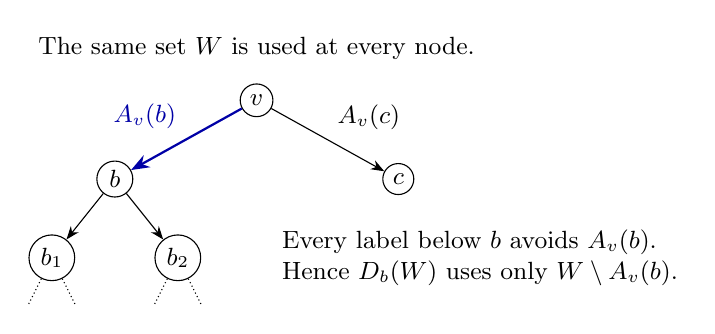
\begin{tikzpicture}[x=1cm,y=1cm,>=Stealth,
  vertex/.style={circle,draw,fill=white,inner sep=2pt},
  every node/.style={font=\small}]
\node[vertex] (v) at (0,0) {$v$};
\node[vertex] (b) at (-1.8,-1.0) {$b$};
\node[vertex] (c) at (1.8,-1.0) {$c$};
\node[vertex] (b1) at (-2.6,-2.0) {$b_1$};
\node[vertex] (b2) at (-1.0,-2.0) {$b_2$};
\draw[->,thick,blue!65!black] (v)--node[above left] {$A_v(b)$} (b);
\draw[->] (v)--node[above right] {$A_v(c)$} (c);
\draw[->] (b)--(b1);
\draw[->] (b)--(b2);
\draw[densely dotted] (b1)--(-2.9,-2.6);
\draw[densely dotted] (b1)--(-2.3,-2.6);
\draw[densely dotted] (b2)--(-1.3,-2.6);
\draw[densely dotted] (b2)--(-0.7,-2.6);
\node[align=left,anchor=west] at (0.2,-2.0)
  {Every label below $b$ avoids $A_v(b)$.\\
   Hence $D_b(W)$ uses only $W\setminus A_v(b)$.};
\node[anchor=south] at (0,0.4) {The same set $W$ is used at every node.};
\end{tikzpicture}
\caption{Disjointness along paths controls the change of measure. Every
arc below $b$ lies on a path through its incoming arc, so the potential
$D_b$ is a function of coordinates outside the incoming label. The diagram
is schematic; labels on different branches may overlap.}
\label{fig:outside}
\end{figure}


In the local transition at $v$,
\[
 t_{vb}(W)\le
 \PP\bigl(\mathrm{target}=b,\ Z(Y)\ge\ee^{-10m_s}\mid W\bigr).
\]
We may consequently apply \eqref{eq:distortion} with $f(W)=D_b(W)$.
Together with \eqref{eq:local-failure} and
$\epsilon_s^{-1}=\ee^{m_s}$, the recurrence gives
\begin{equation}\label{eq:expected-potential}
 \EE D_v(W)
 \le \ee^{-8m_s}
    +\ee^{12m_s}\sum_{b\in\ch(v)}\nu_v(b)\,\EE D_b(W).
\end{equation}
This step controls the dependence caused by reusing $W$.
Since the child weights sum to one, backward induction yields
\[
 \EE D_v(W)\le
 \sum_{j=s}^k
 \exp\left(12\sum_{h=s}^{j-1}m_h-8m_j\right).
\]
In particular, if $o$ is the root, then
\begin{align*}
 \PP(o\text{ is bad})
 &\le\EE D_o(W)\\
 &\le\sum_{j=1}^k
   \exp\left(12\sum_{h<j}m_h-8m_j\right)
 <\tfrac14.
\end{align*}
For the last inequality, geometric growth gives
$\sum_{h<j}m_h\le m_j/15$, and the $m_j$ are distinct positive
integers. Thus the sum is at most
$\sum_{m\ge1}\ee^{-7m}<1/4$.

\medskip\noindent
\textit{The reduced tree.}
On success, start from the good root. At any good node $v$ with
outgoing level $j$, put
\[
 \gamma_v(W)=\sum_{b\ \mathrm{good}}t_{vb}(W)\ge1-\epsilon_j.
\]
Retain each good child $b$ with $t_{vb}(W)>0$, give it weight
$t_{vb}(W)/\gamma_v(W)$, replace its incoming label by
\[
 T_b=A_v(b)\setminus W,
\]
and continue recursively into $b$. The result is a pruned and
reweighted subtree of the input tree. It has the same depth because
$\gamma_v>0$ at every retained non-leaf node. Its labels are subsets
of the old labels, so it is disjoint. Since
$A_v(b)\subseteq W\cup T_b$ on every retained arc, it also satisfies
\eqref{eq:recovery}. A retained child has $t_{vb}>0$, which implies
$|T_b|\le\lfloor m_j/2\rfloor$.

This new child law is the target marginal of the joint transition
conditioned on local non-failure and a good target. Denote this
conditioning event by $E_v$. For the spread bound, use the source:
\eqref{eq:two-inclusions} gives $T\subseteq A_v(c)$ for every
transition, and the unconditioned source has law $\nu_v$ even at fixed
$W$. Thus, for every nonempty $J\subseteq X$,
\begin{align*}
 \PP(J\subseteq T\mid E_v,W)
 &\le\frac{\PP_{c\sim\nu_v}(J\subseteq A_v(c))}{\gamma_v(W)}\\
 &\le\frac{\alpha_j^{|J|}}{1-\epsilon_j}
 \le\left(\frac{\alpha_j}{1-\epsilon_j}\right)^{|J|}.
\end{align*}
This proves all the assertions. The quantities $t_{vb}(W)$ define
the entire construction deterministically; sources and targets are
auxiliary random variables used to analyze its weights.
\end{proof}

\subsection{Iteration}

\begin{proof}[Proof of Theorem~\ref{thm:tree}]
If $r=1$, the conclusion is immediate. Suppose $r<1$, and set
\[
 a=4\sigma,\qquad \rho=\ee^{50}a,
 \qquad s=\lfloor\log_2\ell_k\rfloor+1.
\]
In particular $0<\rho<1$. Start with $\TT$ and make successive
attempts using fresh independent sets of law $\mu_\rho$. A failed attempt leaves
the current tree unchanged. After a successful attempt, retain the
tree provided by Lemma~\ref{lem:reduction}.
Conditionally on the complete past, the current tree is fixed and the
next draw still has law $\mu_\rho$.

After $t$ successes, the capacity at original level $i$ is
\begin{equation}\label{eq:capacities}
 m_i(t)=\left\lfloor\frac{\ell_i}{2^t}\right\rfloor,
\end{equation}
using $\lfloor\lfloor x\rfloor/2\rfloor=\lfloor x/2\rfloor$.
Levels of zero capacity form an initial segment. After each success,
choose any one path through that segment and keep its ending
subtree, deleting the segment. All committed labels are empty, so
each path of the retained subtree extends to a full path by adjoining
the chosen empty prefix. This preserves the recovery guarantee and every
bound at a retained node. If no levels remain, only the root is left.
Fix a tie-breaking rule for these choices. The remaining positive capacities still
satisfy $m_{i+1}(t)\ge16m_i(t)$, since
$\lfloor16x\rfloor\ge16\lfloor x\rfloor$.

At a remaining original level $i$, a valid spread parameter after
$t$ successes is
\begin{equation}\label{eq:spread-iteration}
 \alpha_i(t)=\sigma
 \prod_{u=0}^{t-1}
 \left(1-\ee^{-\lfloor\ell_i/2^u\rfloor}\right)^{-1}.
\end{equation}
The positive integers $\lfloor\ell_i/2^u\rfloor$ in this product are
distinct. The infinite product over all positive integers is less
than $4$, because
\begin{align*}
 \sum_{m=1}^{\infty}-\log(1-\ee^{-m})
 &\le \frac{1}{1-\ee^{-1}}\sum_{m=1}^{\infty}\ee^{-m}\\
 &=\frac{\ee^{-1}}{(1-\ee^{-1})^2}<\log 4.
\end{align*}
Consequently $\alpha_i(t)\le4\sigma=a$. The initial tree satisfies
these bounds, and Lemma~\ref{lem:reduction} proves them inductively
after every success. Thus every attempt before completion has
conditional success probability at least $3/4$.

After $s$ successes, \eqref{eq:capacities} is zero at every level.
Composing \eqref{eq:recovery} through the successful reductions shows
that the union of their draws contains the labels of a path in the
original tree. The expected waiting time for each next success is
at most $4/3$: conditionally on the past, its tail is bounded by
that of a geometric random variable with success probability $3/4$.
Hence the expected number of attempts needed is at most $4s/3$.
By Markov's inequality, completion occurs within $4s$ attempts with
probability at least $2/3$.

Predraw $4s$ independent sets of law $\mu_\rho$, including any that
the procedure ultimately does not use, and take their union $W_* $.
It has law $\mu_{r_*}$, where
\[
 r_*=1-(1-\rho)^{4s}
 \le4s\rho
 =16\ee^{50}\sigma s
 \le16\ee^{50}\sigma(1+\log_2\ell_k)=r.
\]
With probability at least $2/3$, $W_*$ contains a path union.
The same bound holds for $\mu_r$ by monotonicity.
\end{proof}


\section{Application to graph containment}\label{sec:graphs}

It remains to construct the tree required by Theorem~\ref{thm:tree}.
We use the normalized-containment maximization and conditional-extension
argument of Tran~\cite[Section~3, Lemma~3.1]{Tran26}, with constants suited
to the factor-$16$ separation of capacities. The copy-count identity below
also appears in Mossel, Niles-Weed, Sun, and Zadik~\cite[Equation~(5)]{MNSZ22}.

Put $q=\pE(n,H)$ and $\sigma=128q$. Delete the isolated vertices of $H$
and of each graph subsequently considered, and identify these graphs
with their edge sets. This does not change the event of containing
$H$: any copy of its nonisolated part can be extended by choosing the
required number of additional vertices, since $n\ge|V(H)|$ and
copies need not be induced. Every edge subset used below, on its
incident vertices, is a subgraph of the original $H$, so its
expectation at $q$ is at least $1/2$.
Throughout this deletion, $q$ remains the threshold defined using the
original graph $H$.

For a graph $F$ without isolated vertices, let
\[
 M(F)=N(K_n,F),\qquad M(I,F)=N(I,F).
\]
In particular, $M(F)=(n)_{v(F)}/|\operatorname{Aut}(F)|$, where
$(n)_v=n(n-1)\cdots(n-v+1)$ and $\operatorname{Aut}(F)$ is the group of
vertex permutations preserving adjacency. Dividing by this group counts
each ordinary copy once; $M(I,F)$ likewise counts copies, rather than
vertex embeddings.
For the empty edge set use $M(\varnothing)=M(I,\varnothing)=1$.
If $\boldsymbol I$ is a uniformly chosen copy of $I$ on $[n]$, and
$F_0$ is any fixed copy of an edge subset $F\subseteq I$, then
\begin{equation}\label{eq:copy-ratio}
 \PP(F_0\subseteq\boldsymbol I)=\frac{M(I,F)}{M(F)}.
\end{equation}
Indeed, permutation symmetry makes the probability independent of
the chosen copy $F_0$. Summing it over all $M(F)$ copies counts the
$M(I,F)$ copies contained in each $\boldsymbol I$.

\begin{lemma}[Graph hierarchy]\label{lem:hierarchy}
There is a disjoint probability tree on
$X=\binom{[n]}2$ whose path unions are copies of $H$ with its isolated
vertices removed, such that every level is $\sigma$-spread and its label
sizes $\ell_1,\ldots,\ell_k$ satisfy
\[
 1\le\ell_1,\qquad \ell_{i+1}\ge16\ell_i,
 \qquad \ell_k\le e(H).
\]
\end{lemma}

\begin{proof}
For a current nonempty edge set $I\subseteq H$, choose an edge
subset $S\subseteq I$ maximizing
\begin{equation}\label{eq:maximizer}
 R_\sigma(I,S)=\sigma^{-|S|}\PP(S_0\subseteq\boldsymbol I),
\end{equation}
where $S_0$ is any fixed copy of $S$ on $[n]$. The empty set is
allowed and has value $1$. Fix any deterministic rule for breaking
ties.

Write $h_I=|I|$ and $r=|S|>0$. The expectation constraint gives
$M(S)q^r\ge1/2$, while $M(I,S)\le\binom{h_I}{r}$.
By \eqref{eq:copy-ratio},
\[
 R_\sigma(I,S)\le2\binom{h_I}{r}(q/\sigma)^r
           =2\binom{h_I}{r}128^{-r}.
\]
For $r\ge h_I/17$, the bound
$\binom{h_I}{r}\le(\ee h_I/r)^r$ gives
\[
 R_\sigma(I,S)\le2(17\ee/128)^r<1.
\]
Thus every maximizing predecessor satisfies $|S|<|I|/17$.

Repeat the selection until the empty set is reached, and write
the resulting nested sequence in reverse order as
\[
 \varnothing=H_0\subset H_1\subset\cdots\subset H_k=H,
 \qquad |H_{i-1}|<|H_i|/17.
\]
Here and below $H$ denotes its edge set. Build a tree rooted at the
empty set. From each reached copy $S_0$ of $H_{i-1}$, take as
children all copies of $H_i$ containing $S_0$, with the uniform
distribution, and label the arc to a child $I_0$ by $I_0\setminus S_0$.
Such children exist, since every copy of $H_{i-1}$ extends to a copy
of $H_i$ on $[n]$. Keep distinct histories as distinct tree nodes.
The labels on every path are disjoint and their union is a copy of
$H$. Their sizes are
\[
 \ell_i=|H_i|-|H_{i-1}|>0,
 \qquad
 \ell_{i+1}>16|H_i|\ge16\ell_i.
\]

It remains to check conditional spread. At a node $S_0$, let $A$
be its random added label. If $J\cap S_0\ne\varnothing$, then
$\PP(J\subseteq A)=0$. Otherwise, for a uniform copy
$\boldsymbol I$ of $H_i$,
\begin{equation}\label{eq:conditional-ratio}
 \PP(J\subseteq A)=
 \frac{\PP(S_0\cup J\subseteq\boldsymbol I)}
      {\PP(S_0\subseteq\boldsymbol I)}.
\end{equation}
If the numerator is positive, $S_0\cup J$ is isomorphic to an edge
subset $U\subseteq H_i$. Maximality of $H_{i-1}$ in
\eqref{eq:maximizer} gives
\[
 \sigma^{-(|S_0|+|J|)}\PP(S_0\cup J\subseteq\boldsymbol I)
 \le \sigma^{-|S_0|}\PP(S_0\subseteq\boldsymbol I).
\]
Together with \eqref{eq:conditional-ratio}, this gives
$\PP(J\subseteq A)\le\sigma^{|J|}$. If the numerator is zero, the same
bound is immediate. This proves the lemma.
\end{proof}

\begin{proof}[Proof of Theorem~\ref{thm:main}]
Apply Theorem~\ref{thm:tree} to the tree of
Lemma~\ref{lem:hierarchy}, with $\sigma=128q$. Since
$\ell_k\le h=e(H)$, a Bernoulli edge set with parameter
\[
 r=\min\{1,\;2048\ee^{50}q(1+\log_2 h)\}
\]
contains a copy of $H$ with probability at least $2/3$. This proves
\eqref{eq:stronger}. Finally, $h\le\binom n2\le n^2$ and $n\ge2$
give $1+\log_2 h\le3\log_2 n$, and hence the stated constant
$C=6144\ee^{50}$.
\end{proof}


\begin{thebibliography}{99}
\raggedright

\bibitem{ALWZ21}
R.~Alweiss, S.~Lovett, K.~Wu, and J.~Zhang,
\emph{Improved bounds for the sunflower lemma},
Annals of Mathematics (2) \textbf{194} (2021), no.~3, 795--815.
\href{https://doi.org/10.4007/annals.2021.194.3.5}{doi:10.4007/annals.2021.194.3.5}.

\bibitem{Bollobas81}
B.~Bollob\'as,
\emph{Threshold functions for small subgraphs},
Mathematical Proceedings of the Cambridge Philosophical Society
\textbf{90} (1981), no.~2, 197--206.
\href{https://doi.org/10.1017/S0305004100058655}{doi:10.1017/S0305004100058655}.

\bibitem{DKP25}
Q.~Dubroff, J.~Kahn, and J.~Park,
\emph{On the ``second'' Kahn--Kalai conjecture},
arXiv:2508.14269v1 (August 19, 2025).
\url{https://arxiv.org/abs/2508.14269v1}.

\bibitem{DKP25Cases}
Q.~Dubroff, J.~Kahn, and J.~Park,
\emph{On the ``second'' Kahn--Kalai conjecture: cliques, cycles, and trees},
arXiv:2510.02005v2 (October 23, 2025).
\url{https://arxiv.org/abs/2510.02005v2}.

\bibitem{ER60}
P.~Erd\H{o}s and A.~R\'enyi,
\emph{On the evolution of random graphs},
Publications of the Mathematical Institute of the Hungarian Academy of
Sciences \textbf{5} (1960), 17--61.
\url{https://static.renyi.hu/~p_erdos/1960-10.pdf}.

\bibitem{ER66}
P.~Erd\H{o}s and A.~R\'enyi,
\emph{On the existence of a factor of degree one of a connected random graph},
Acta Mathematica Academiae Scientiarum Hungaricae
\textbf{17} (1966), 359--368.
\url{https://users.renyi.hu/~p_erdos/1966-16.pdf}.

\bibitem{FKNP21}
K.~Frankston, J.~Kahn, B.~Narayanan, and J.~Park,
\emph{Thresholds versus fractional expectation-thresholds},
Annals of Mathematics (2) \textbf{194} (2021), no.~2, 475--495.
\href{https://doi.org/10.4007/annals.2021.194.2.2}{doi:10.4007/annals.2021.194.2.2}.

\bibitem{KK07}
J.~Kahn and G.~Kalai,
\emph{Thresholds and expectation thresholds},
Combinatorics, Probability and Computing
\textbf{16} (2007), no.~3, 495--502.
\href{https://doi.org/10.1017/S0963548307008474}{doi:10.1017/S0963548307008474}.

\bibitem{LSZ19}
S.~Lovett, N.~Solomon, and J.~Zhang,
\emph{From DNF compression to sunflower theorems via regularity},
34th Computational Complexity Conference, LIPIcs \textbf{137} (2019),
5:1--5:14.
\href{https://doi.org/10.4230/LIPIcs.CCC.2019.5}{doi:10.4230/LIPIcs.CCC.2019.5}.

\bibitem{MNSZ25}
E.~Mossel, J.~Niles-Weed, N.~Sun, and I.~Zadik,
\emph{A Bayesian proof of the spread lemma},
Random Structures \& Algorithms \textbf{66} (2025), no.~4, e70008.
\href{https://doi.org/10.1002/rsa.70008}{doi:10.1002/rsa.70008}.

\bibitem{MNSZ22}
E.~Mossel, J.~Niles-Weed, N.~Sun, and I.~Zadik,
\emph{On the second Kahn--Kalai conjecture},
arXiv:2209.03326v1 (September 7, 2022).
\url{https://arxiv.org/abs/2209.03326v1}.

\bibitem{OpenAIThresholdEquivalence2026}
OpenAI,
\emph{Integral and fractional expectation thresholds are equivalent},
OpenAI Math Release preprint
\href{https://github.com/openai/math/blob/main/preprints/Integral-and-fractional-expectation-thresholds-are-equivalent-September-23-2026/paper.pdf}{OAI:Integral-and-fractional-expectation-thresholds-are-equivalent-September-23-2026},
2026, Theorem~1.1, p.~2.

\bibitem{PP24}
J.~Park and H.~T.~Pham,
\emph{A proof of the Kahn--Kalai conjecture},
Journal of the American Mathematical Society
\textbf{37} (2024), no.~1, 235--243.
\href{https://doi.org/10.1090/jams/1028}{doi:10.1090/jams/1028}.

\bibitem{Riordan00}
O.~Riordan,
\emph{Spanning subgraphs of random graphs},
Combinatorics, Probability and Computing
\textbf{9} (2000), no.~2, 125--148.
\href{https://doi.org/10.1017/S0963548399004150}{doi:10.1017/S0963548399004150}.

\bibitem{Tal10}
M.~Talagrand,
\emph{Are many small sets explicitly small?},
Proceedings of the 42nd ACM Symposium on Theory of Computing (2010),
13--36.
\href{https://doi.org/10.1145/1806689.1806693}{doi:10.1145/1806689.1806693}.

\bibitem{Tran26}
T.~Tran,
\emph{Fractional expectation thresholds and the ``second'' Kahn--Kalai
conjecture},
arXiv:2609.20546v2 (September 24, 2026).
\url{https://arxiv.org/abs/2609.20546v2}.

\end{thebibliography}

\end{document}
